\documentclass[12pt]{article}


% -------------------- PAQUETES --------------------
\usepackage[utf8]{inputenc}
\usepackage[spanish]{babel}
\usepackage[margin=2.54cm]{geometry}
\usepackage{graphicx}
\usepackage{xcolor}


% -------------------- CARGA DE ARCHIVOS EXTERNOS --------------------
% ----------------- UTILIDADES PARA DAR UN MEJOR FORMATO DE DOCUMENTO -----------------  


\definecolor{azul}{rgb}{0.0039, 0.3098, 0.6196}


% Formato para el indice general ...........
\makeatletter
    \renewcommand{\@dotsep}{1.5}
    \renewcommand{\l@section}{\@dottedtocline{1}{1.5em}{2.3em}}
    \renewcommand{\l@subsection}{\@dottedtocline{2}{3.8em}{3.2em}}
    \renewcommand{\l@subsubsection}{\@dottedtocline{3}{7.0em}{4.1em}}
\makeatother

% --------- COMANDOS PERSONALIZADOS PARA LA PORTADA DE LAS TAREAS, TRABAJOS Y PROYECTOS ---------

\newcommand{\rutaLogo}[1]{\newcommand{\RutaLogo}{#1}}
\newcommand{\tema}[1]{\newcommand{\Tema}{#1}}
\newcommand{\etiquetaAutores}[1]{\newcommand{\EtiquetaAutores}{#1}}
\newcommand{\alumno}[1]{\newcommand{\Alumno}{#1}}
\newcommand{\materia}[1]{\newcommand{\Materia}{#1}}
\newcommand{\docente}[1]{\newcommand{\Docente}{#1}}
\newcommand{\ciclo}[1]{\newcommand{\Ciclo}{#1}}
\newcommand{\fecha}[1]{\newcommand{\Fecha}{#1}}
\newcommand{\periodo}[1]{\newcommand{\Periodo}{#1}}



% -------------------- DEFINICIÓN DE LA PORTADA --------------------
\rutaLogo{../../../RecursosGlobales/Img/logo_tec_azuay.png}
\tema{\\ \vspace{1cm} Guía Práctica N°1 - Introducción a la lógica proposicional: conceptos y estructuras básicas  \\ \vspace{1.7cm}}
\etiquetaAutores{Alumno:}
\alumno{Eduardo Mendieta \vspace{1cm}}
\materia{Matemática \vspace{1cm}}
\docente{Lcda. Vilma Duchi, Mgtr. \vspace{1cm}}
\ciclo{Primer Ciclo - M1A \vspace{1.1cm}}
\fecha{16 de junio de 2024 \vspace{1cm}}
\periodo{Abril 2024 - Agosto 2024}



% -------------------- INFORME --------------------
\begin{document}

    \begin{titlepage}

    \centering

    \includegraphics[width=0.11\textwidth]{\RutaLogo} 

    \vspace{0.3cm}
    \textcolor{azul}{\Large \textbf{Instituto Superior Universitario Tecnológico del Azuay \\}}
    \vspace{0.3cm}
    \textcolor{azul}{\Large \textbf{Tecnología Superior en Big Data}}
    
    % 1. ---------------- TEMA -------------------------
    
    {\Large\textbf{\Tema}}
    
    % 2. ---------------- AUTOR(ES) -------------------------
    \textcolor{azul}{\large \textbf{\EtiquetaAutores} \\}
    \vspace{0.3cm}
    {\large \Alumno}

    % 3. ---------------- MATERIA -------------------------
    \textcolor{azul}{\large \textbf{Materia:} \\}
    \vspace{0.3cm}
    {\large \Materia}


    % 3. ---------------- DOCENTE -------------------------
    \textcolor{azul}{\large \textbf{Docente:} \\}
    \vspace{0.3cm}
    {\large \Docente}


    % 3. ---------------- Ciclo -------------------------
    \textcolor{azul}{\large \textbf{Ciclo:} \\}
    \vspace{0.3cm}
    {\large \Ciclo}


    % 3. ---------------- FECHA -------------------------
    \textcolor{azul}{\large \textbf{Fecha:} \\}
    \vspace{0.3cm}
    {\large \Fecha}

    % 3. ---------------- PERIODO -------------------------
    \textcolor{azul}{\large \textbf{Periodo Académico:} \\}
    \vspace{0.3cm}
    {\large \Periodo}
 
\end{titlepage}

  
    \section*{\centering Guía práctica N°1 - Unidad 2\\Aplicaciones Prácticas}

        \vspace{0.6cm}
        \begin{itemize}
            % PARTE 1: -----------------------------------------------------
            \item \textbf{Problemas de la Vida Real:} \\Aplicar la lógica proposicional para modelar y resolver 3 problemas de la vida cotidiana. Una vez modelada las situaciones elabore la tabla de verdad y en otro apartado simplifique las aplicando las leyes de lógica proposicional.
                \begin{enumerate}
                    % Ejercicio N°1: ..........................................
                    \item Si aprobamos la materia de Matemática Discreta, entonces significa que estudiamos la teoría de lógica proposicional. Pero no estudiamos la teoría de lógica proposicional y si aprobamos la materia de Matemática Discreta, entonces tuvimos suerte.
                        \par$p:$ Aprobamos la materia de Matemática Discreta.
                        \par$q:$ Estudiamos la teoría de lógica proposicional.
                        \par$r:$ Tuvimos suerte.
                        \par$n = 3$, $2^n = 2^3 = 8.$ \vspace{0.5cm}
                        \par\textbf{Proposición: }$(p \longrightarrow q) \wedge [(\sim q \wedge p) \longrightarrow r]$\vspace{0.5cm}

                        \begin{figure}[!h]
                            \centering
                            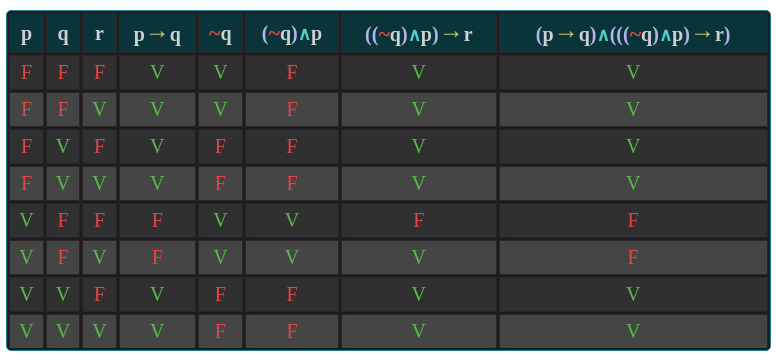
\includegraphics[width=0.7\textwidth]{Img/Tarea8_a_ej1.png}
                        \end{figure} \vspace{0.5cm}

                        \par{\large$(p \longrightarrow q) \wedge [(\sim q \wedge p) \longrightarrow r]$} \vspace{0.5cm}
                        \par$(\sim p \vee q) \wedge [\sim (\sim q \wedge p) \vee r]$ {\footnotesize Leyes condicionales.}
                        \par$(\sim p \vee q) \wedge [(q \vee \sim p) \vee r]$ {\footnotesize Leyes de Morgan e involución.}
                        \par$(\sim p \vee q) \wedge [(\sim p \vee q) \vee r]$ {\footnotesize Leyes asociativas.}
                        \par$\sim p \vee q$ {\footnotesize Leyes de absorción.} \vspace{0.5cm}
                        \par\textbf{Respuesta: } la proposición es una contingencia. \vspace{0.5cm}

                        
                    % Ejercicio N°2: ..........................................
                    \newpage
                    \item Si hemos dormido las 8 horas reglamentarias, entonces tenemos mucha energía y aprobaremos el examen con un 10. Pero no es cierto que tengamos mucha energía o que aprobemos el examen con un 10, entonces no hemos dormido las 8 horas reglamentarias.
                        \par$p:$ Hemos dormido las 8 horas reglamentarias.
                        \par$q:$ Tenemos mucha energía.
                        \par$r:$ Aprobamos el examen con un 10.
                        \par$n = 3$, $2^n = 2^3 = 8.$ \vspace{0.5cm}
                        \par\textbf{Proposición: }$[p \longrightarrow (q \wedge r)] \wedge [\sim (q \vee r) \longrightarrow \sim p]$\vspace{0.5cm}

                        \begin{figure}[!h]
                            \centering
                            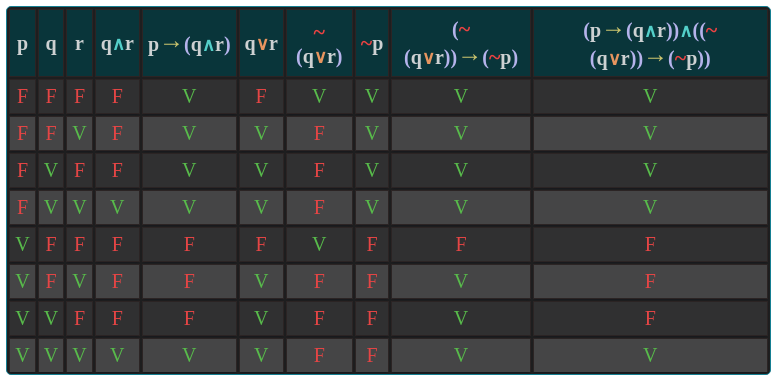
\includegraphics[width=0.7\textwidth]{Img/Tarea8_a_ej2.png}
                        \end{figure} \vspace{0.5cm}

                        \par{\large$[p \longrightarrow (q \wedge r)] \wedge [\sim (q \vee r) \longrightarrow \sim p]$} \vspace{0.5cm}
                        \par$[\sim p \vee (q \wedge r)] \wedge [(q \vee r) \vee \sim p]$ {\footnotesize Leyes condicionales e involución.}
                        \par$\sim p \vee [(q \wedge r) \wedge (q \vee r)]$ {\footnotesize Leyes distributivas.}
                        \par$\sim p \vee [q \wedge (r \wedge (r \vee q))]$ {\footnotesize Leyes asociativas.}
                        \par$\sim p \vee (q \wedge r)$ {\footnotesize Leyes de absorción.} \vspace{0.5cm}
                        \par\textbf{Respuesta: } la proposición es una contingencia. \vspace{0.5cm}

                   
                    % Ejercicio N°3: ..........................................
                    \newpage
                    \item Ganaré la competencia de 5k organizada por los estudiantes de entrenamiento deportivo si y solo si entreno todos los días por una hora. Tuve mucha fatiga durante la carrera y no logré llegar a la meta primero. En conclusión, como no cumplí con el entrenamiento, entonces tuve dicha fatiga y por lo tanto no gané la competencia.
                        \par$p:$ Gane la competencia de 5k organizada por los estudiantes de entrenamiento deportivo.
                        \par$q:$ Entrene todos los días por una hora.
                        \par$r:$ Tuve mucha fatiga durante la carrera.
                        \par$n = 3$, $2^n = 2^3 = 8.$ \vspace{0.5cm}
                        \par\textbf{Proposición: }$[(p \leftrightarrow q) \wedge (r \wedge \sim p)] \longrightarrow [\sim q \longrightarrow (r \wedge \sim p)]$\vspace{0.5cm}

                        \begin{figure}[!h]
                            \centering
                            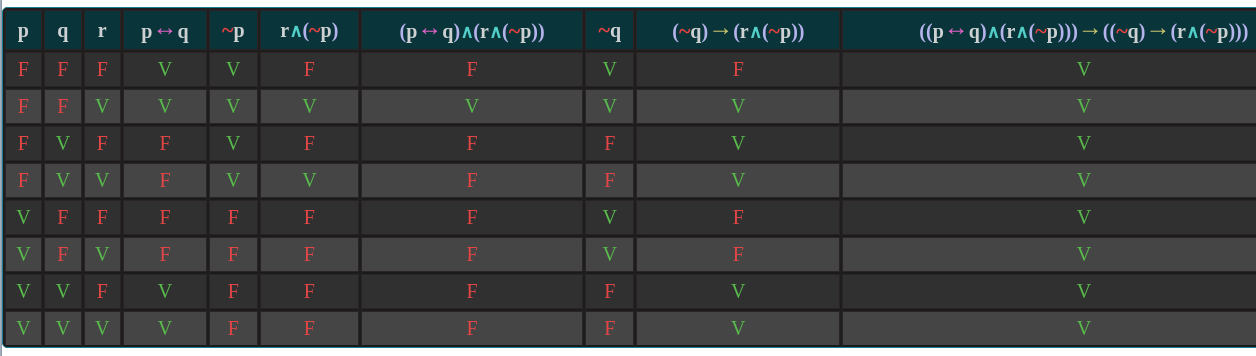
\includegraphics[width=0.9\textwidth]{Img/Tarea8_a_ej3.png}
                        \end{figure} \vspace{0.5cm}

                        \par{\large$[(p \leftrightarrow q) \wedge (r \wedge \sim p)] \longrightarrow [\sim q \longrightarrow (r \wedge \sim p)]$} \vspace{0.5cm}
                        \par$[[(p \longrightarrow q) \wedge (q \longrightarrow p)] \wedge (r \wedge \sim p)] \longrightarrow [\sim q \longrightarrow (r \wedge \sim p)]$ {\footnotesize Leyes bicondicionales.}
                        \par$[[(\sim p \vee q) \wedge (\sim q \vee p)] \wedge (r \wedge \sim p)] \longrightarrow [q \vee (r \wedge \sim p)]$ {\footnotesize Leyes condicionales e involución.}
                        \par$\sim [[(\sim p \vee q) \wedge (\sim q \vee p)] \wedge (r \wedge \sim p)] \vee [q \vee (r \wedge \sim p)]$ {\footnotesize Leyes condicionales.}
                        \par$[\sim [(\sim p \vee q) \wedge  (\sim q \vee p)] \vee \sim (r \wedge \sim p)] \vee [q \vee (r \wedge \sim p)]$ {\footnotesize Leyes de Morgan.}
                        \par$[[\sim (\sim p \vee q) \vee \sim (\sim q \vee p)] \vee (\sim r \vee  p)] \vee [q \vee (r \wedge \sim p)]$ {\footnotesize Leyes de Morgan.}
                        \par$[[(p \wedge \sim q) \vee  (q \wedge \sim p)] \vee (\sim r \vee  p)] \vee [q \vee (r \wedge \sim p)]$ {\footnotesize Leyes de Morgan.}
                        \par$p \vee (p \wedge \sim q)  \vee (q \wedge \sim p) \vee (r \wedge \sim p) \vee \sim r  \vee q$ {\footnotesize Leyes asociativas.}
                        \par$p  \vee  \sim p \wedge (q \vee r) \vee \sim r  \vee q$ {\footnotesize Leyes de absorción y distributivas.}
                        \par$V \wedge (q \vee r) \vee \sim r  \vee q$  {\footnotesize Leyes del tercio excluido.}
                        \par$q \vee r \vee \sim r  \vee q$ {\footnotesize Formas normales.}
                        \par$(r \vee \sim r) \vee (q \vee q)$ {\footnotesize Leyes asociativas.}
                        \par$V \vee q$ {\footnotesize Leyes del tercio excluido e idempotencia.}
                        \par$V$ {\footnotesize Formas normales.} \vspace{0.5cm}
                        \par\textbf{Respuesta: } la proposición es una Tautología. \vspace{0.5cm}
                
                \end{enumerate}
            
            % PARTE 2: -----------------------------------------------------
            \newpage
            \item \textbf{ Poner en práctica lo aprendido: Modelar las situaciones en expresiones lógicas.}\\ Dadas las siguientes situaciones formalice a lenguaje proposicional y elabore las tablas de verdad: 
            
            \begin{enumerate}
                % Ejercicio N°1: ..........................................
                \item Para que se organice un evento exitoso en un parque, se deben cumplir varias condiciones: debe ser un día soleado, los permisos del gobierno deben estar aprobados, el equipo de sonido debe estar disponible y el catering debe estar confirmado. Además, si llueve, el evento se trasladará a un auditorio, pero solo si el auditorio está disponible.
                
                % Ejercicio N°2: ..........................................
                \item Para que un proyecto de investigación sea aceptado, debe cumplir con ciertos criterios: el proyecto debe ser innovador, debe contar con la aprobación del comité de ética, y debe tener financiamiento asegurado. Además, si el proyecto involucra experimentación con humanos, debe tener la autorización de los sujetos participantes y el respaldo de un hospital.
                
                % Ejercicio N°3: ..........................................
                \item Para ser admitido en un programa de posgrado, un estudiante debe tener una licenciatura, haber pasado un examen de admisión, y contar con una carta de recomendación de un profesor. Además, si el estudiante no tiene una licenciatura en el campo específico del programa, debe haber completado cursos de nivelación.
                
                % Ejercicio N°4: ..........................................
                \item Para implementar una plataforma de análisis de Big Data, se deben cumplir varias condiciones: el almacenamiento debe estar configurado, los datos deben estar limpios y preparados, el equipo de análisis debe estar capacitado, y las herramientas de visualización deben estar integradas. Además, si los datos incluyen información sensible, se deben cumplir las normativas de privacidad y seguridad.
                
                % Ejercicio N°5: ..........................................
                \item Una empresa desea predecir la demanda de sus productos para optimizar su cadena de suministro. Para ello, deben cumplirse las siguientes condiciones:
                    \begin{itemize}
                        \item Los datos históricos de ventas deben estar disponibles.
                        \item Si la demanda de un producto ha aumentado en los últimos 3 meses, se considera una tendencia al alza.
                        \item Si la demanda de un producto ha disminuido en los últimos 3 meses, se considera una tendencia a la baja.
                        \item Se desea identificar los productos que tienen una tendencia al alza y una tendencia a la baja para ajustar la producción.
                    \end{itemize}
            \end{enumerate}
        \end{itemize}
\end{document}